\section[Le problème]{Le problème~--- tout le monde sait ce qu'est une carte, personne ne peut la définir}

L'intuition commune ne pose pas de problème. Face à une carte routière, une carte du ciel ou un plan d'occupation des sols, l'identification est immédiate et unanime : c'est une carte. La difficulté commence dès que l'on sort de ces cas prototypiques.

Un plan de métro est-il une carte ? Il représente bien un réseau de transport dans l'espace d'une ville, mais il en déforme délibérément la géographie~--- les distances entre stations ne correspondent à aucune réalité métrique, et l'échelle n'est pas respectée. Une carte mentale (\textit{mind map}) est-elle une carte ? Elle organise des concepts dans un espace visuel, mais sans référent territorial. Une cartographie bibliométrique, qui positionne des articles scientifiques selon leurs proximités thématiques (figure~\ref{fig:bibliometric}), mérite-t-elle l'appellation ? Et les arbres généalogiques, représentations structurées des relations génétiques au sein d'une famille, pourquoi les exclut-on instinctivement, alors qu'ils satisfont pourtant les deux premiers critères identifiés en prologue ?

\begin{figure}[ht]
  \centering
  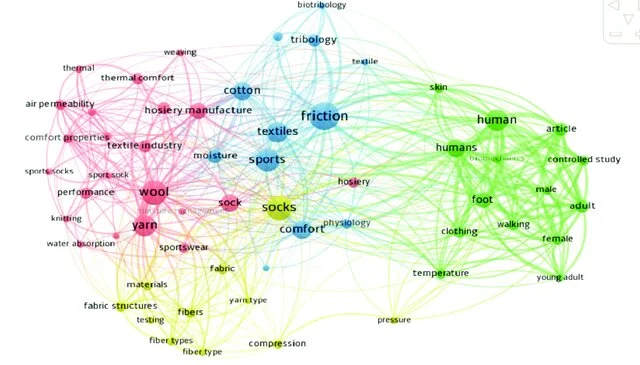
\includegraphics[width=0.72\textwidth]{Figures/bibliometric_map.png}
  \caption{Carte bibliométrique des co-occurrences de mots-clés dans la littérature sur les chaussettes de sport. Les couleurs indiquent des communautés thématiques~; la proximité encode la similarité sémantique. \protect\parencite[fig.~5]{moraMunoz2025}}
  \label{fig:bibliometric}
\end{figure}

Le critère de densité semblait apporter une réponse à cette accumulation d'exemples. Il capturait une intuition réelle : quelque chose change quand un graphe devient très connecté. Mais l'examen des cas concrets contredit cette intuition. Un organigramme peut être très ramifié, comporter des connexions transversales entre départements (figure~\ref{fig:arbre_organigramme}), et rester indéniablement un organigramme. À l'inverse, une carte routière représentant une région peu peuplée peut ne comporter que quelques routes et quelques carrefours, et rester indéniablement une carte. La densité ne discrimine pas.

\begin{figure}[ht]
\centering
\begin{subfigure}[b]{0.42\textwidth}
  \centering
  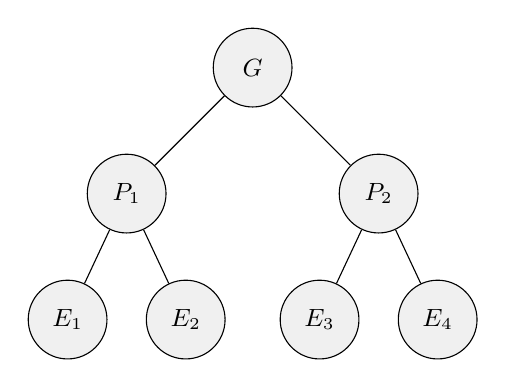
\begin{tikzpicture}[
    every node/.style={circle, draw, fill=gray!12, minimum size=1cm, font=\small},
    level 1/.style={sibling distance=3.2cm, level distance=1.6cm},
    level 2/.style={sibling distance=1.5cm, level distance=1.6cm}
  ]
  \node {$G$}
    child { node {$P_1$}
      child { node {$E_1$} }
      child { node {$E_2$} }
    }
    child { node {$P_2$}
      child { node {$E_3$} }
      child { node {$E_4$} }
    };
  \end{tikzpicture}
  \caption{Arbre généalogique}
\end{subfigure}
\hfill
\begin{subfigure}[b]{0.52\textwidth}
  \centering
  \begin{tikzpicture}[
    box/.style={rectangle, draw, fill=gray!12, minimum width=1.7cm,
                minimum height=0.75cm, font=\small},
    arr/.style={-{Stealth[length=2.5mm]}, semithick},
    node distance=0pt
  ]
  \node[box] (dir) {PDG};
  \node[box, below left=1.4cm and 1.8cm of dir]  (d1) {Dép.\ A};
  \node[box, below right=1.4cm and 1.8cm of dir] (d2) {Dép.\ B};
  \node[box, below=1.4cm of d1] (a1) {Agent 1};
  \node[box, below=1.4cm of d2] (a2) {Agent 2};
  \draw[arr] (dir) -- (d1);
  \draw[arr] (dir) -- (d2);
  \draw[arr] (d1)  -- (a1);
  \draw[arr] (d2)  -- (a2);
  \draw[arr, dashed] (a1) to[bend right=22] (a2);
  \end{tikzpicture}
  \caption{Organigramme}
\end{subfigure}
\caption{Deux structures relationnelles qui ne sont pas des cartes. Dans les deux cas, la position verticale encode un niveau hiérarchique, non une proximité entre éléments. La flèche en pointillé illustre qu'ajouter des connexions transversales ne suffit pas à transformer la structure en carte.}
\label{fig:arbre_organigramme}
\end{figure}

La situation est plus nuancée pour les réseaux. Les visualisations de réseaux sociaux ou d'internet constituent en effet un cas intéressant : lorsqu'un algorithme de mise en page regroupe spatialement les n\oe{}uds fortement connectés, des régions émergent, des communautés se dessinent, et l'on parle spontanément de \emph{cartographier} le réseau. Ce glissement de vocabulaire n'est pas anodin~--- il signale que quelque chose de proprement cartographique apparaît, mais seulement sous certaines conditions. Un réseau représenté sous forme de matrice d'adjacence ou de liste d'arêtes n'est pas une carte. Le même réseau, visualisé par un algorithme de spatialisation qui traduit la similarité structurelle en proximité visuelle, peut le devenir. La différence n'est pas dans les données~--- elle est dans la façon dont l'espace visuel est mis en relation avec elles.

Ce que ces exemples révèlent collectivement est le suivant. Dans un arbre ou un organigramme, les relations encodées sont des relations entre éléments adjacents : A est connecté à B, B est connecté à C. La position d'un n\oe{}ud dans l'espace visuel ne porte pas d'information en elle-même~--- ce qui compte, c'est avec quels autres éléments il est relié. Sur une carte, en revanche, la position relative de deux éléments dit quelque chose même en l'absence de connexion explicite entre eux. Deux villes sans route directe ont néanmoins une relation de voisinage, une direction relative, une distance implicite. Ce n'est pas la densité des connexions qui fait la carte~--- c'est la nature de ce que l'espace visuel encode.

Cette observation conduit à reformuler la question. Ce n'est pas le nombre de relations qui distingue la carte du graphe, mais le fait que la carte encode un espace dans lequel la position elle-même est porteuse de sens~--- un espace dans lequel on peut se situer, estimer des distances, inférer des relations entre éléments qui ne sont pas explicitement reliés. Préciser la nature de cet espace est l'objet de la section suivante.